\documentclass[10pt]{article}
\usepackage{preamble}
\usepackage[T1]{fontenc}   % keeps underscores selectable when the PDF text is copied
\usepackage{amsmath}
\usepackage{booktabs}
\usepackage{float}
\usepackage{graphicx}
% Required for inserting images


\renewcommand\thesubsection{\Alph{subsection}}



\begin{document}

\begin{titlepage}
    \begin{center}
        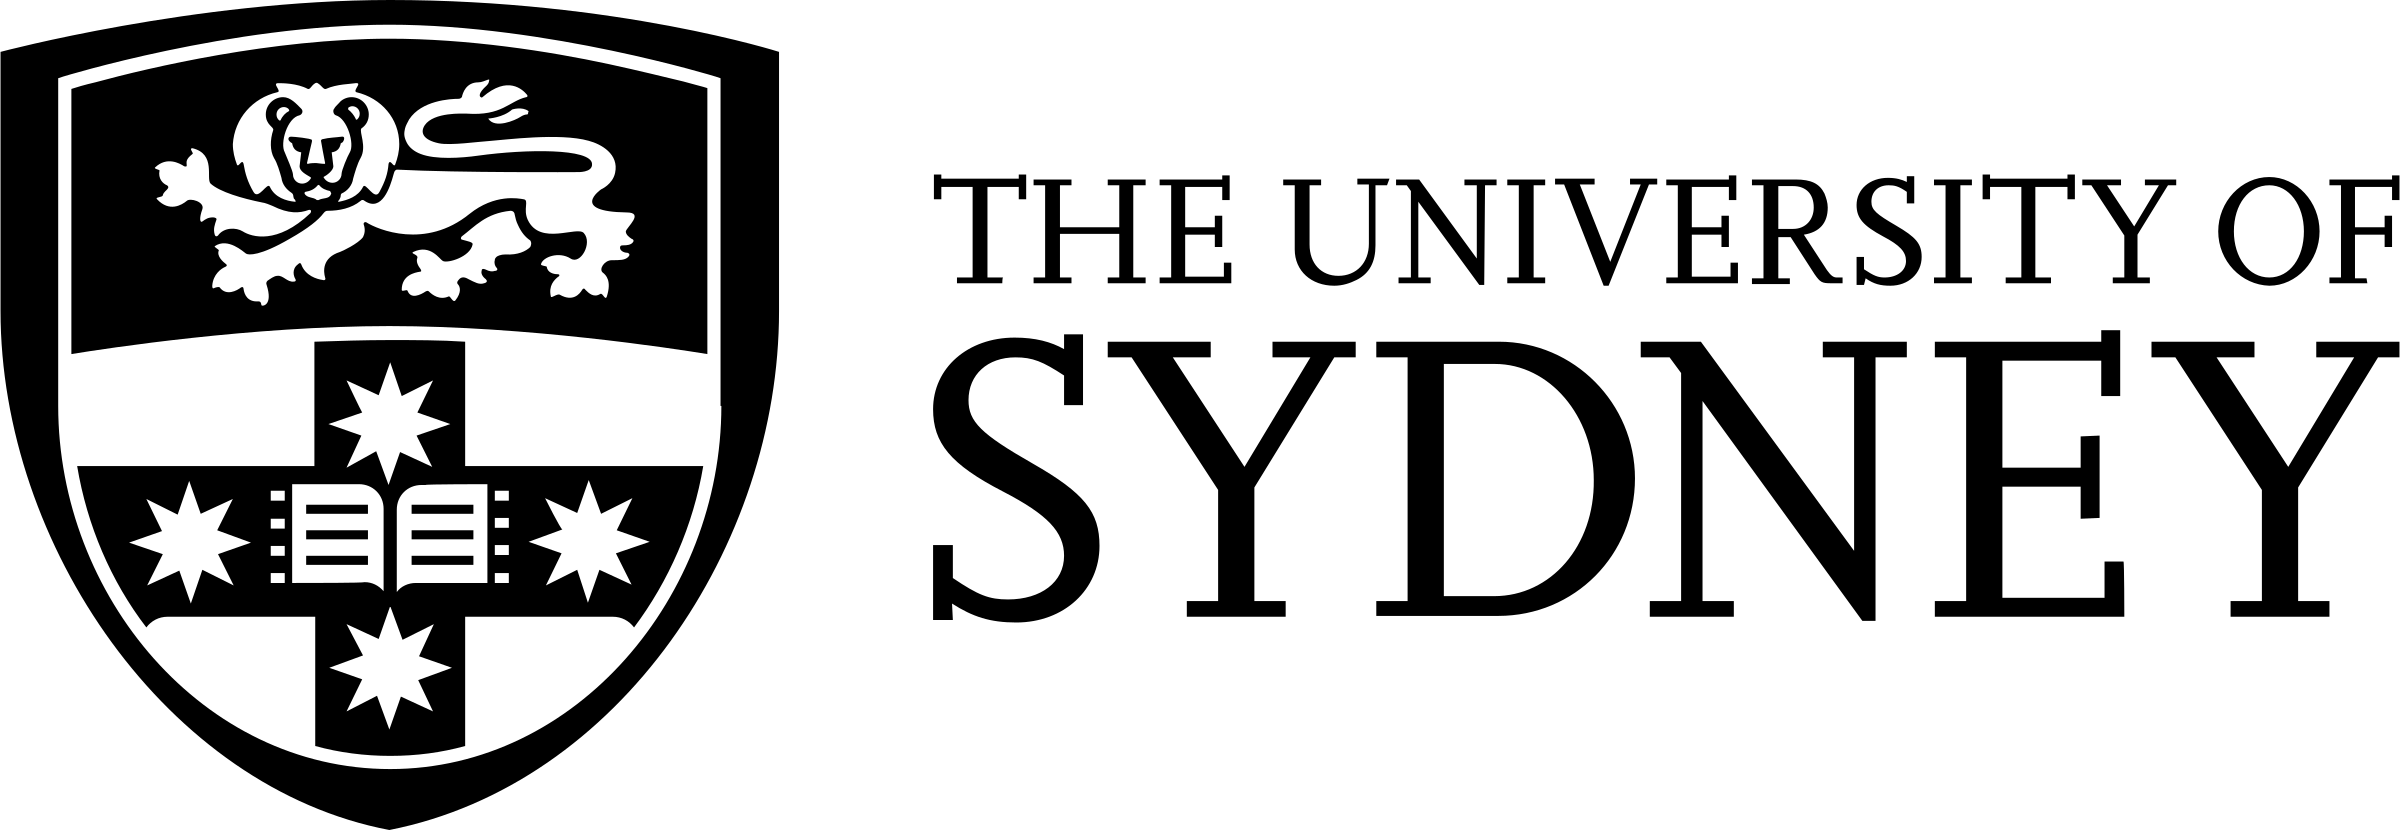
\includegraphics[width=0.5\textwidth]{image/usydNew.png}\\[3cm]
    \end{center}
    \begin{center}
        \textsc{\LARGE The University of Sydney}\\[0.8cm]
        \textsc{\Large The University of Sydney Engineering School}\\[1cm]
        \textsc{\Large MTRX3760: Mechatronic Systems Design}\\[1cm]
        \HRule \\[1cm]
        {\huge \textbf{Lab 2 --- Robot Simulator}}\\[1cm]
        \HRule \\[1cm]
    \end{center}

    \begin{center}
        \textsc{\Large \textbf{530544164}}\\[0.5cm]      %%% TODO check SIDs
        \textsc{\Large \textbf{550777766}}\\[1cm]
        \textsc{\large Practical Section 3 --- Friday 9\,am}\\[1.5cm]   %%% TODO check section
    \end{center}

    \begin{center}
       \textsc{\large Semester 2, 2026}\\[1.5cm]          %%% TODO check semester
    \end{center}
    \vfill
\end{titlepage}
\tableofcontents

\newpage
\null % Holds the page open
\thispagestyle{empty}

%=============================================================================
\section{A0 Team Setup}
%=============================================================================

\subsection{Main strength relevant to this lab}
\textbf{530544164 ---} %%% TODO one or two sentences
\\[0.3cm]
\textbf{550777766 ---} %%% TODO one or two sentences

\subsection{Main area for improvement relevant to this lab}
\textbf{530544164 ---} %%% TODO one or two sentences
\\[0.3cm]
\textbf{550777766 ---} %%% TODO one or two sentences

\subsection{How we arrive at decisions, and resolve disagreements}
%%% TODO. Worth mentioning, if true: design decisions settled before any code
%%% is written; disagreements resolved by writing both options down and
%%% comparing them against the unit's design principles rather than by
%%% seniority; whoever owns a file has the final say on its internals.

\subsection{How we keep on schedule}
%%% TODO. Worth mentioning, if true: the work was split into A1 first,
%%% then A2 built on top of it, with the functionality hurdle cleared before
%%% any code-quality work began; a checkpoint before the lab session each week.

\subsection{Revision control and code review}
We use Git, hosted on GitHub, for all source code. The repository holds
\texttt{A1/} and \texttt{A2/} as separate directories so that the A1
submission is preserved intact while A2 is built on top of a copy of it, as
the assignment requires.

Code review happens on merge: every change is read by the member who did not
write it before it reaches the main branch, using \texttt{git diff}. The
reason is the one given in lectures --- it is easier to write code than to
debug it, and a second reader catches inconsistencies far more cheaply than a
debugger does. Build artefacts (\texttt{*.o} and the linked executables) are
excluded from version control, since only source belongs in the repository.

%%% TODO adjust the paragraph above if your workflow differs.


%=============================================================================
\section{A1 Wall Follower}
%=============================================================================

\subsection{Design}

The simulator is built from twelve classes in four layers. The lowest layer is
the supplied code: \texttt{CRender}, which is the only place in the program
that raylib is named, and \texttt{CLoopReader}, which parses a map file into a
start pose and a list of vertices.

Above that sits the world. \texttt{CSegmentLoop} turns a vertex list into a
closed loop of straight segments and answers two purely geometric questions:
how far along a ray the first segment lies, and how far a point is from the
nearest segment. It knows nothing about walls, robots or sensors.
\texttt{CRoom} wraps one \texttt{CSegmentLoop} and gives it meaning ---
something a sensor ray can meet, and something a robot's body can collide
with. The vector arithmetic both rely on is collected as static methods on
\texttt{CVecMath}, which holds no state and is omitted from the diagram to
keep it readable.

The robot layer is where the design does most of its work.
\texttt{CRobot} is an abstract base class holding everything every robot has:
a pose, a \texttt{CDifferentialDrive} carrying two \texttt{CWheel} objects, a
\texttt{CTrail}, and an update counter. Its \texttt{Update()} is deliberately
\emph{not} virtual. It fixes the order of a simulation step --- decide wheel
speeds, drive, count, react, record the trail --- and exposes exactly two
hooks: a pure virtual \texttt{ComputeWheelSpeeds()} that a concrete robot must
supply, and a virtual \texttt{OnAfterMove()} it may override. A derived class
therefore cannot forget a step or reorder one; it can only fill in the
decisions that are genuinely its own. \texttt{CWallFollowerRobot} fills both
hooks, owns its two \texttt{CRangeSensor} objects, and \emph{knows} the
\texttt{CRoom} without owning it.

At the top, \texttt{CSimulation} owns the window, the map reader, the room and
the robots, and drives them through a fixed number of fixed-length simulated
timesteps. It only ever calls \texttt{CRobot}'s interface, so it needs no
change at all when a second kind of robot is added in A2.

\begin{figure}[H]
    \centering
    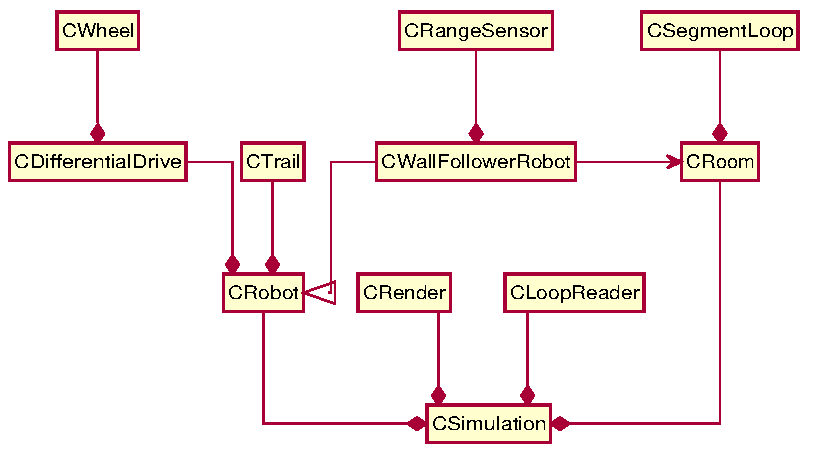
\includegraphics[width=\textwidth]{image/A1_uml.pdf}
    \caption{A1 class diagram. Filled diamonds mark composition (the diamond
    sits at the owner), the hollow triangle marks inheritance, and the open
    arrow marks association.}
\end{figure}

Three decisions are worth setting out explicitly.

\textbf{Wheels are objects, not numbers.} The assignment specifies two
independently controlled wheels, so each is a \texttt{CWheel} that is
commanded a speed and reports how far it rolls in a given time. The clamp on
a commanded speed lives inside the wheel, so no controller can ask for a speed
the motor could not deliver.

\textbf{The heading convention is left-handed.} The renderer's $y$ axis grows
downward and \texttt{CPose} measures its heading clockwise from $+x$, so the
usual differential-drive formula changes sign: the robot's angular rate is
$(v_{\text{left}} - v_{\text{right}}) / L$, not the other way round. Driving
the left wheel faster turns the robot to its right, as it would in reality.
This was verified before any control code was written.

\textbf{The start heading in the map file is taken at face value.}
\texttt{SimpleWalls.map} carries a comment saying the robot starts facing
right, but its \texttt{startpose 150 140 90} means facing \emph{down} under
the documented convention. The data is the sensible one: facing down puts the
left wall 50 units off the robot's right-hand side, which is a proper
wall-following start, whereas facing right would leave the nearest wall on
that side 360 units away. The parsed data was used and the comment treated as
stale.

\subsection{Control strategy}

The right-facing sensor gives a distance error against a target standoff. The
forward-right sensor anticipates corners: against a straight wall parallel to
the robot it must read $\sqrt{2}$ times the right sensor, so the difference
between what it reads and that expectation says whether the wall ahead is
turning in or falling away. The two errors are combined proportionally and
clamped. When both sensors report their maximum range the wall has been lost
around an outside corner, and the robot turns hard toward where it should be
until a sensor finds it again. There is no integral or derivative term; the
room is a small polygon and a proportional law with corner anticipation was
enough to complete the circuit without touching a wall.

\subsection{Screenshot}

\begin{figure}[H]
    \centering
    \includegraphics[width=\textwidth]{image/A1_screenshot.png}
    \caption{The wall follower after one complete circuit of
    \texttt{SimpleWalls.map}. The blue curve is the stored trail, the two
    amber rays are the range sensors, and the short black line on the body is
    the heading indicator.}
\end{figure}

\subsection{Console output}

The run completed with no collisions, so no collision lines were printed. Had
the robot touched a wall, each contact would have produced one line naming the
update it happened on.

\begin{verbatim}
Run summary
Updates completed : 2000
Total collisions  : 0
\end{verbatim}

A collision is counted on the update it begins, not on every update the body
is still overlapping a wall, so one contact of any duration reports once.


%=============================================================================
\section{A2 Line Follower}
%=============================================================================

\subsection{Design}

A2 adds three classes and extends one. Eleven of A1's files are used
unchanged.

\texttt{CFloorLine} is the counterpart of \texttt{CRoom}: it wraps the same
\texttt{CSegmentLoop}, built from \texttt{SimpleLine.map}, and answers the one
question a floor sensor asks --- whether a point lies on the line. Treating
the line as five units wide reduces to testing whether the point is within
half that of the centreline, which is exactly the point-to-segment distance
\texttt{CSegmentLoop} already computed for collision detection in A1.

\texttt{CLineSensor} differs from \texttt{CRangeSensor} in both what it
reports and how it is mounted. It returns a boolean rather than a distance,
and it is fixed at an offset \emph{position} --- so far forward, so far to the
right --- rather than at an angle, because a floor sensor looks at the patch
of floor beneath it rather than along a ray.

\texttt{CLineFollowerRobot} derives from the same \texttt{CRobot} and fills
the same \texttt{ComputeWheelSpeeds()} hook. It does not override
\texttt{OnAfterMove()}, because it has no collisions to count.

\texttt{CSimulation} is the one A1 class that had to change: it now reads two
map files and owns a \texttt{CFloorLine} alongside the \texttt{CRoom}, and its
single start-pose accessor became two, since the robots start in different
places. Its run loop was not touched.

\begin{figure}[H]
    \centering
    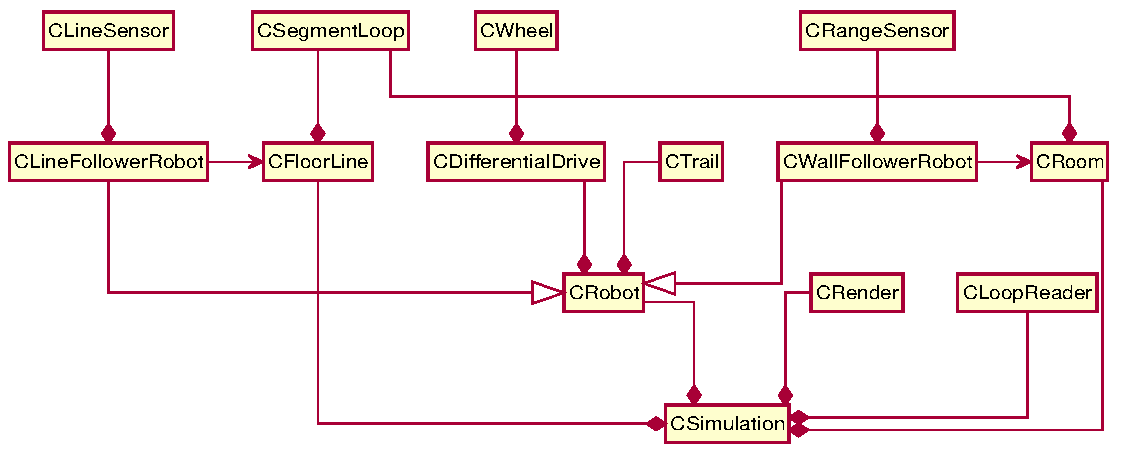
\includegraphics[width=\textwidth]{image/A2_uml.pdf}
    \caption{A2 class diagram. Both robots derive from the same
    \texttt{CRobot}; \texttt{CRoom} and \texttt{CFloorLine} are built on the
    same \texttt{CSegmentLoop}.}
\end{figure}

\subsection{Control strategy}

The line follower hugs the right-hand edge of the line rather than its centre,
which turns two boolean readings into a usable error signal. One sensor sits
on the robot's centreline, the other just outside the line to its right. Both
on means the robot has drifted right and is pulled back; centre off and edge
on means it has drifted left and steers back in; centre on and edge off is the
intended state and the robot drives straight. Both off means the line has been
lost at a corner, and the robot turns tightly until it crosses the line again.

\subsection{Screenshot}

\begin{figure}[H]
    \centering
    \includegraphics[width=\textwidth]{image/A2_screenshot.png}
    \caption{Both robots after completing their circuits. Blue is the wall
    follower's trail, orange is the line follower's, and the yellow band is
    the floor line drawn at its real five-unit width. The small loops in the
    orange trail are the line follower reacquiring the line after a sharp
    corner.}
\end{figure}

\subsection{Console output}

\begin{verbatim}
Run summary
Updates completed        : 3500
Wall follower collisions : 0
\end{verbatim}


%=============================================================================
\section{A3 Post-Mortem}
%=============================================================================

\subsection{Individual contributions}
\textbf{530544164 ---} %%% TODO what did this member contribute
\\[0.3cm]
\textbf{550777766 ---} %%% TODO what did this member contribute

\subsection{One thing each of us would improve about the Team Setup}
\textbf{530544164 ---} %%% TODO
\\[0.3cm]
\textbf{550777766 ---} %%% TODO

\subsection{An important aspect of A1's design we had to change for A2}

\texttt{CSimulation}. In A1 it knew about exactly one piece of scenery, the
room, and offered one start pose. A2 needed a second piece of scenery with a
different meaning and a second start position, so the constructor now takes
both map filenames, the class owns a \texttt{CFloorLine} as well as a
\texttt{CRoom}, and \texttt{GetStartPose()} became
\texttt{GetWallStartPose()} and \texttt{GetLineStartPose()}.

The change was contained because ownership was already clear: \texttt{main}
had no scenery to rearrange, and no robot held a pointer into anything it did
not own.

\subsection{An important aspect of A1's design that turned out well for A2}

Two, and they are the same idea at different levels.

\texttt{CSegmentLoop} was written to know nothing about what its segments
represent. That looked like an extra layer in A1, where the only loop was a
wall. In A2 the floor line is also a closed loop of straight segments, so
\texttt{CFloorLine} reuses the class without a line of change --- and
the point-to-segment distance written for collision detection is exactly what
the five-unit line-width test needs.

\texttt{CRobot::Update()} being non-virtual, with a pure virtual
\texttt{ComputeWheelSpeeds()} as its only required hook, meant writing the
line follower came down to filling in one function. The motion, the trail, the
update count and the drawing of the body all came across untouched, and there
was no opportunity to get the order of a simulation step wrong.

\subsection{One aspect of the submitted programs' structure we are happy with}

The ownership chain is unambiguous and matches the object model.
\texttt{CSimulation} owns the window, the scenery and the robots and deletes
them in its destructor; a robot owns its drive, its wheels, its sensors and
its trail; a robot only \emph{knows} the room or the line it senses. Because
robots are deleted through a \texttt{CRobot*}, the virtual destructor on the
base class is doing real work rather than being a formality.

\subsection{One aspect of the structure we would most want to improve}

\texttt{CSimulation} exposes \texttt{GetRoom()}, \texttt{GetFloorLine()} and
the two start poses purely so that \texttt{main} can construct robots against
them. That is four accessors that exist for one caller, and it leaks a little
of the simulation's internals. A better arrangement would let a robot be
registered with the pieces of the world it needs, rather than having the
caller fetch them first.

\subsection{One aspect of the submitted programs' style we are happy with}

Constants live with the class that owns them. Every magic number in the
program has a name and is a private \texttt{static const} member of the class
whose behaviour it describes --- the target wall distance and the two steering
gains belong to the wall follower, the wall colour and thickness to the room,
the parallel tolerance to the geometry. Nothing sits at file scope, and both
programs compile without a single warning under
\texttt{-Wall -Wextra -Wshadow -Wnon-virtual-dtor -pedantic}.

\subsection{One aspect of the style we would most want to improve}

\texttt{CWallFollowerRobot::Draw()} reads both range sensors again in order to
draw their rays, having already read them in \texttt{ComputeWheelSpeeds()}
during the same step. The readings are identical, so nothing is wrong, but the
same call is written twice for two different reasons. Caching the readings
taken during the update and drawing those would be both cheaper and clearer.


%=============================================================================
\section{A4 ROS Tutorials}
%=============================================================================

%%% TODO


%=============================================================================
\section{A5 Noise Bonus}
%=============================================================================

%%% TODO


%=============================================================================
\section{Self-Assessment}
%=============================================================================

%%% TODO revise these numbers before submitting. Do not include the
%%% self-assessment bonus itself in the estimate.

\begin{table}[H]
\centering
\begin{tabular}{lr}
\toprule
Component & Estimated mark \\
\midrule
Functionality       & Pass \\
A0 Team Setup       & 8 / 10\\
Design Quality      & 26 / 30\\
Code Quality        & 26 / 30\\
A3 Post-Mortem      & 8 / 10\\
A4 ROS Tutorials    & 18 / 20\\
A5 Noise Bonus      & 0 / +10\\
\midrule
\textbf{Total}      & \textbf{86 / 100}\\
\bottomrule
\end{tabular}
\end{table}


%=============================================================================
\section{Code Appendix}
%=============================================================================

All source code written for this assignment, as text. A1 and A2 are submitted
as separate directories so that the A1 program is preserved in full; the
eleven files A2 shares with A1 are identical in both and are listed once,
under A1.

\begingroup
\setstretch{1}
\lstset{
  basicstyle=\ttfamily\footnotesize,
  breaklines=true,
  breakatwhitespace=false,
  postbreak=\mbox{$\hookrightarrow$\space},
  columns=fullflexible,
  keepspaces=true,
  showstringspaces=false,
  tabsize=2,
  commentstyle=\ttfamily,
  keywordstyle=\ttfamily\bfseries,
  stringstyle=\ttfamily,
  frame=none,
  numbers=left,
  numberstyle=\ttfamily\scriptsize,
  numbersep=6pt,
  xleftmargin=18pt,
  aboveskip=0.6em,
  belowskip=1.2em,
}

\subsection*{A1 Wall Follower}
\addcontentsline{toc}{subsection}{A1 Wall Follower}

\noindent\textbf{\ttfamily\small A1/main.cpp}
\lstinputlisting[language=C++]{code/A1/main.cpp}

\noindent\textbf{\ttfamily\small A1/CSimulation.h}
\lstinputlisting[language=C++]{code/A1/CSimulation.h}

\noindent\textbf{\ttfamily\small A1/CSimulation.cpp}
\lstinputlisting[language=C++]{code/A1/CSimulation.cpp}

\noindent\textbf{\ttfamily\small A1/CRobot.h}
\lstinputlisting[language=C++]{code/A1/CRobot.h}

\noindent\textbf{\ttfamily\small A1/CRobot.cpp}
\lstinputlisting[language=C++]{code/A1/CRobot.cpp}

\noindent\textbf{\ttfamily\small A1/CWallFollowerRobot.h}
\lstinputlisting[language=C++]{code/A1/CWallFollowerRobot.h}

\noindent\textbf{\ttfamily\small A1/CWallFollowerRobot.cpp}
\lstinputlisting[language=C++]{code/A1/CWallFollowerRobot.cpp}

\noindent\textbf{\ttfamily\small A1/CDifferentialDrive.h}
\lstinputlisting[language=C++]{code/A1/CDifferentialDrive.h}

\noindent\textbf{\ttfamily\small A1/CDifferentialDrive.cpp}
\lstinputlisting[language=C++]{code/A1/CDifferentialDrive.cpp}

\noindent\textbf{\ttfamily\small A1/CWheel.h}
\lstinputlisting[language=C++]{code/A1/CWheel.h}

\noindent\textbf{\ttfamily\small A1/CWheel.cpp}
\lstinputlisting[language=C++]{code/A1/CWheel.cpp}

\noindent\textbf{\ttfamily\small A1/CRangeSensor.h}
\lstinputlisting[language=C++]{code/A1/CRangeSensor.h}

\noindent\textbf{\ttfamily\small A1/CRangeSensor.cpp}
\lstinputlisting[language=C++]{code/A1/CRangeSensor.cpp}

\noindent\textbf{\ttfamily\small A1/CRoom.h}
\lstinputlisting[language=C++]{code/A1/CRoom.h}

\noindent\textbf{\ttfamily\small A1/CRoom.cpp}
\lstinputlisting[language=C++]{code/A1/CRoom.cpp}

\noindent\textbf{\ttfamily\small A1/CSegmentLoop.h}
\lstinputlisting[language=C++]{code/A1/CSegmentLoop.h}

\noindent\textbf{\ttfamily\small A1/CSegmentLoop.cpp}
\lstinputlisting[language=C++]{code/A1/CSegmentLoop.cpp}

\noindent\textbf{\ttfamily\small A1/CVecMath.h}
\lstinputlisting[language=C++]{code/A1/CVecMath.h}

\noindent\textbf{\ttfamily\small A1/CVecMath.cpp}
\lstinputlisting[language=C++]{code/A1/CVecMath.cpp}

\noindent\textbf{\ttfamily\small A1/CTrail.h}
\lstinputlisting[language=C++]{code/A1/CTrail.h}

\noindent\textbf{\ttfamily\small A1/CTrail.cpp}
\lstinputlisting[language=C++]{code/A1/CTrail.cpp}

\noindent\textbf{\ttfamily\small A1/Makefile}
\lstinputlisting[language=make]{code/A1/Makefile.txt}

\newpage

\subsection*{A2 Line Follower}
\addcontentsline{toc}{subsection}{A2 Line Follower}

Only the files that differ from A1, or that do not exist in A1, are listed
here.

\noindent\textbf{\ttfamily\small A2/main.cpp}
\lstinputlisting[language=C++]{code/A2/main.cpp}

\noindent\textbf{\ttfamily\small A2/CSimulation.h}
\lstinputlisting[language=C++]{code/A2/CSimulation.h}

\noindent\textbf{\ttfamily\small A2/CSimulation.cpp}
\lstinputlisting[language=C++]{code/A2/CSimulation.cpp}

\noindent\textbf{\ttfamily\small A2/CFloorLine.h}
\lstinputlisting[language=C++]{code/A2/CFloorLine.h}

\noindent\textbf{\ttfamily\small A2/CFloorLine.cpp}
\lstinputlisting[language=C++]{code/A2/CFloorLine.cpp}

\noindent\textbf{\ttfamily\small A2/CLineSensor.h}
\lstinputlisting[language=C++]{code/A2/CLineSensor.h}

\noindent\textbf{\ttfamily\small A2/CLineSensor.cpp}
\lstinputlisting[language=C++]{code/A2/CLineSensor.cpp}

\noindent\textbf{\ttfamily\small A2/CLineFollowerRobot.h}
\lstinputlisting[language=C++]{code/A2/CLineFollowerRobot.h}

\noindent\textbf{\ttfamily\small A2/CLineFollowerRobot.cpp}
\lstinputlisting[language=C++]{code/A2/CLineFollowerRobot.cpp}

\noindent\textbf{\ttfamily\small A2/build.sh}
\lstinputlisting[language=bash]{code/A2/build.sh}

\newpage

\endgroup

\end{document}
